\section{推理}

\begin{logicbox}[title=引言]
\textit{推理是逻辑学的实践应用,通过系统化的思考方法和训练,我们能够解决复杂问题并发展批判性思维能力。}
\end{logicbox}

如前所述,逻辑学是研究用于区分正确推理与不正确推理的方法和原理的学问。\logicterm{推理}与\logicterm{论证}都是从已知前提(或为特定目的而假定的前提)推出结论的思维过程。

到目前为止,我们主要专注于分析和评估他人的论证。然而,在日常生活中,我们每天都需要\logicemph{建构自己的论证}:
\begin{itemize}
  \item 决定自己的行动方案
  \item 评价他人的行为
  \item 为道德或政治信念进行辩护
  \item 解决复杂的实际问题
\end{itemize}

\logicwarn{建构和运用优质论证的技能具有巨大价值},这种技能直接影响我们的决策质量和说服能力。

\begin{theorembox}[title=推理技能的培养]
\logicemph{训练方法}:
\begin{itemize}
  \item \logicterm{推理游戏}:国际象棋、围棋、Mastermind等策略游戏
  \item \logicterm{逻辑谜题}:专门设计的推理问题
  \item \logicterm{实际应用}:日常问题的系统分析
\end{itemize}

\logicemph{双重价值}:
\begin{itemize}
  \item \logicterm{实用价值}:提高问题解决能力
  \item \logicterm{娱乐价值}:享受思维挑战的乐趣
\end{itemize}
\end{theorembox}

正如美国哲学家约翰·杜威所说:"\logicemph{对思虑的享受是受过训练的大脑的标志}"。推理既是必要的生存技能,也是令人愉悦的智力活动。

\begin{theorembox}[title=人工设计问题与现实问题的对比]
\logicemph{人工设计问题的特点}:
\begin{itemize}
  \item \logicterm{结构简洁}:信息明确,条件清晰
  \item \logicterm{逻辑纯粹}:专注于推理技巧本身
  \item \logicterm{答案确定}:存在明确的解决方案
\end{itemize}

\logicemph{解决策略}:
\begin{itemize}
  \item \logicterm{系统推理}:构建推理链条,将中间结论作为后续前提
  \item \logicterm{创造性重组}:对已知信息进行新的组合和理解
  \item \logicterm{持续探索}:面对困难时保持耐心和毅力
\end{itemize}

\logicwarn{思维模式的相似性}:解决逻辑谜题的思考方式与侦探、新闻工作者、陪审员的推理过程本质相同。
\end{theorembox}

虽然人工设计的问题有时会让人无功而返,但\logicemph{通过成功的推理应用解决问题时带来的满足感是无与伦比的}。这种智力挑战不仅锻炼了我们的逻辑思维能力,也为我们提供了纯粹的智力娱乐。

\footnotetext{(1)种著名的网络智力游戏。
}

\subsection{推理问题的类型与解法}

推理问题中最常见的类型是\logicterm{身份识别问题},这类问题要求我们仅凭提供的线索来确定相关人物的身份、角色或其他属性。

\begin{examplebox}[title=航班乘务员职务分配问题]
\begin{displayquote}
在某个航班的全体乘务员中,飞机驾驶员、副驾驶员和飞行工程师的职务由爱伦、布朗和卡尔三人担任,但不必是这个次序。\\
副驾驶员是个独生子,钱挣得最少。\\
卡尔与布朗的姐姐结了婚,钱挣得比驾驶员多。\\
问:三个人每人担任什么职务?
\end{displayquote}
\end{examplebox}

\begin{theorembox}[title=解题策略:排除法推理]
\logicemph{第一步:寻找突破口}
寻找信息最丰富的对象。从前提可知关于卡尔的多个条件:
\begin{itemize}
  \item 卡尔挣得比驾驶员多 → \logicwarn{卡尔不是驾驶员}
  \item 副驾驶员挣得最少,而卡尔挣得比驾驶员多 → \logicwarn{卡尔不是副驾驶员}
  \item 通过排除法 → \logicterm{卡尔是飞行工程师}
\end{itemize}

\logicemph{第二步:利用中间结论}
已知卡尔是飞行工程师,继续分析布朗:
\begin{itemize}
  \item 布朗有姐姐,副驾驶员是独生子 → \logicwarn{布朗不是副驾驶员}
  \item 卡尔已是飞行工程师 → \logicwarn{布朗不是飞行工程师}
  \item 通过排除法 → \logicterm{布朗是驾驶员},\logicterm{爱伦是副驾驶员}
\end{itemize}
\end{theorembox}

\subsection{矩阵分析法}

对于复杂的推理问题,我们需要更系统的分析工具。\logicterm{矩阵分析法}是一种强大的图示技术,它能够:
\begin{itemize}
  \item 系统地记录所有可能的选择
  \item 清晰地显示已知信息和推导结论
  \item 避免信息混乱和遗漏
  \item 支持复杂的多步推理
\end{itemize}

\begin{examplebox}[title=四位艺术家身份识别问题]
\begin{displayquote}
阿伦佐、库特、鲁道夫和威拉德是四个天资极高的创造性的艺术家。一个是舞蹈家,一个是画家,一个是歌唱家,一个是作家,但不必是这个次序。\\
(1)那天晚上歌唱家在音乐会舞台上进行他的首次演出时,阿伦佐和鲁道夫在观众席上。\\
(2)库特和作家两人有画家为他们画的生活肖像。\\
(3)作家正准备写一本阿伦佐的传记,他写的威拉德的传记是畅销书。\\
(4)阿伦佐从未听说过鲁道夫。\\
问:每个人的艺术领域是什么?
\end{displayquote}
\end{examplebox}

\begin{theorembox}[title=矩阵法的优势]
\logicemph{信息管理挑战}:
\begin{itemize}
  \item 需要记住多个前提中的众多事实
  \item 需要跟踪从前提推出的中间结论
  \item 便条记录可能导致混乱和遗漏
\end{itemize}

\logicemph{矩阵法的解决方案}:
\begin{itemize}
  \item \logicterm{系统化存储}:为所有相关信息提供结构化空间
  \item \logicterm{动态更新}:随着推理进展不断填入新信息
  \item \logicterm{全局视野}:同时显示所有可能性和已确定结论
\end{itemize}
\end{theorembox}

这个问题的矩阵表必须是显示这四个人(用四行表示)和他们从事的四种艺术职业(用四列表示)的一个列阵,如下所示:

\begin{center}
\begin{tabular}{|l|l|l|l|l|}
\hline
 & 舞蹈家 & 画家 & 歌唱家 & 作家 \\
\hline
阿伦佐 &  &  &  &  \\
\hline
库 特 &  &  &  &  \\
\hline
鲁道夫 &  &  &  &  \\
\hline
威拉徳 &  &  &  &  \\
\hline
\end{tabular}
\end{center}

\begin{theorembox}[title=矩阵填写规则]
\logicemph{符号约定}:
\begin{itemize}
  \item \logicwarn{N}(或"-"):表示"不可能",某人不可能从事某职业
  \item \logicterm{Y}(或"+"):表示"确定",某人确定从事某职业
\end{itemize}

\logicemph{填写策略}:
\begin{enumerate}
  \item 从前提直接推出的否定信息先填入N
  \item 通过排除法确定的肯定信息填入Y
  \item 一旦确定某人的职业,在该行其他位置填入N,在该列其他位置填入N
\end{enumerate}
\end{theorembox}

\logicemph{第一轮分析}:根据前提直接推导
\begin{itemize}
  \item 前提(1):阿伦佐和鲁道夫在观众席 → \logicwarn{都不是歌唱家}
  \item 前提(2):库特和作家有画家画的肖像 → \logicwarn{库特既非画家也非作家}
  \item 前提(3):作家写阿伦佐和威拉德的传记 → \logicwarn{作家既非阿伦佐也非威拉德}
\end{itemize}

第一轮填写后的矩阵表:

\begin{center}
\begin{tabular}{|l|l|l|l|l|}
\hline
 & 舞蹈家 & 画家 & 歌唱家 & 作家 \\
\hline
阿伦佐 &  &  & N & N \\
\hline
库 特 &  & N &  & N \\
\hline
鲁道夫 &  &  & N &  \\
\hline
威拉德 &  &  &  & N \\
\hline
\end{tabular}
\end{center}

\logicemph{第二轮分析}:运用排除法进行深度推理

\begin{theorembox}[title=关键推理步骤]
\logicemph{步骤1:确定鲁道夫的职业}
\begin{itemize}
  \item 观察作家列:阿伦佐(N)、库特(N)、鲁道夫(?)、威拉德(N)
  \item 通过排除法 → \logicterm{鲁道夫必须是作家}
  \item 填入Y,并在鲁道夫行的其他位置填入N
\end{itemize}

\logicemph{步骤2:排除阿伦佐为画家}
\begin{itemize}
  \item 前提(2):鲁道夫有画家画的肖像
  \item 前提(4):阿伦佐从未听说过鲁道夫
  \item 逻辑推理:如果阿伦佐是画家,他应该认识鲁道夫
  \item 结论 → \logicwarn{阿伦佐不可能是画家}
\end{itemize}

\logicemph{步骤3:连锁推理}
\begin{itemize}
  \item 阿伦佐只剩舞蹈家 → \logicterm{阿伦佐是舞蹈家}
  \item 库特只剩歌唱家 → \logicterm{库特是歌唱家}
  \item 威拉德只剩画家 → \logicterm{威拉德是画家}
\end{itemize}
\end{theorembox}

完成的矩阵表:

\begin{center}
\begin{tabular}{|c|c|c|c|c|}
\hline
 & 舞蹈家 & 画家 & 歌唱家 & 作家 \\
\hline
阿伦佐 & Y & N & N & N \\
\hline
库 特 & N & N & Y & N \\
\hline
鲁道夫 & N & N & N & Y \\
\hline
威拉德 & N & Y & N & N \\
\hline
\end{tabular}
\end{center}

\logicemph{最终答案}:从完成的矩阵表可以直接读出:
\begin{itemize}
  \item \logicterm{阿伦佐}是舞蹈家
  \item \logicterm{库特}是歌唱家
  \item \logicterm{鲁道夫}是作家
  \item \logicterm{威拉德}是画家
\end{itemize}

\begin{theorembox}[title=矩阵法的适用性]
\logicemph{复杂问题的处理}:
\begin{itemize}
  \item 当问题涉及多个维度的分类时,矩阵法变得更加复杂但仍然有效
  \item 某些高难度的逻辑问题\logicwarn{几乎不可能}在不使用矩阵方法的情况下解决
  \item 矩阵法提供了系统化的思维框架,避免遗漏和错误
\end{itemize}
\end{theorembox}

\subsection{称重问题:不同类型的推理挑战}

除了身份识别问题,还有其他类型的推理挑战。下面是一个经典的\logicterm{称重问题},它需要不同的解题策略。

\begin{examplebox}[title=六球称重问题]
\logicemph{问题设定}:
\begin{itemize}
  \item 六个球:两个红球(R1, R2)、两个绿球(G1, G2)、两个蓝球(B1, B2)
  \item 每对同色球中,一个重一个轻
  \item 所有重球重量相同,所有轻球重量相同
  \item 球的外观难以区分
  \item 只有一架天平,最多称重两次
\end{itemize}

\logicemph{挑战}:如何识别出每对球中的重球和轻球?
\end{examplebox}

这类问题需要\logicterm{策略性思维}:我们必须设计称重方案,使得每种可能的结果都能提供足够的信息来解决问题。

\begin{theorembox}[title=称重问题解答策略]
\logicemph{第一次称量方案}:$\mathbf{R1 + G1 \text{ vs } R2 + B1}$

\logicemph{情况一:两边平衡}
\begin{itemize}
  \item \logicterm{逻辑分析}:由于R1和R2分别在两边,且两边平衡,说明每边都是"重球+轻球"
  \item \logicterm{推论}:G1和B1必须一重一轻(否则无法平衡)
  \item \logicterm{第二次称量}:$\mathbf{G1 \text{ vs } B1}$
    \begin{itemize}
      \item 如果G1沉下去:G1重(G2轻),B1轻(B2重),R1轻(R2重)
      \item 如果G1升上去:G1轻(G2重),B1重(B2轻),R1重(R2轻)
    \end{itemize}
\end{itemize}

\logicemph{情况二:$R1+G1$沉下去}
\begin{itemize}
  \item \logicterm{关键推理}:如果R1是轻球,那么R2是重球,$R1+G1$不可能沉下去
  \item \logicterm{结论}:R1必须是重球,R2是轻球
\end{itemize}
\end{theorembox}

已知R1是重球后,G1和B1的组合只有三种可能:

\begin{theorembox}[title=可能的组合分析]
\logicemph{三种可能组合}:
\begin{itemize}
  \item (a) G1轻,B1轻
  \item (b) G1重,B1重
  \item (c) G1重,B1轻
\end{itemize}

\logicemph{第二次称量方案}:$\mathbf{R1 + R2 \text{ vs } G1 + B1}$

\logicemph{结果分析}:
\begin{itemize}
  \item \logicterm{如果$R1+R2$沉下去}:
    \begin{itemize}
      \item 重+轻 > G1+B1,说明G1+B1都是轻球
      \item 对应组合(a):G1轻(G2重),B1轻(B2重)
    \end{itemize}
  \item \logicterm{如果$R1+R2$升上去}:
    \begin{itemize}
      \item 重+轻 < G1+B1,说明G1+B1都是重球
      \item 对应组合(b):G1重(G2轻),B1重(B2轻)
    \end{itemize}
  \item \logicterm{如果两边平衡}:
    \begin{itemize}
      \item 重+轻 = 重+轻,说明G1+B1也是一重一轻
      \item 对应组合(c):G1重(G2轻),B1轻(B2重)
    \end{itemize}
\end{itemize}
\end{theorembox}

\logicwarn{解题关键}:通过巧妙设计的两次称重,我们能够在所有可能情况下都获得完整的信息,这体现了\logicemph{策略性推理}的重要性。

\subsection{回溯分析问题}

在现实世界中,我们经常需要从当前状态推断其起因,从现在的情况推出过去的状况。

\logicterm{回溯分析}是从当前状态推断其历史成因的推理过程。这种推理在科学研究中极为重要:

\begin{theorembox}[title=回溯分析的应用领域]
\logicemph{科学应用}:
\begin{itemize}
  \item \logicterm{考古学家}:从文物推断古代文明
  \item \logicterm{地质学家}:从地层推断地球历史
  \item \logicterm{天文学家}:从观测数据推断宇宙演化
  \item \logicterm{医学家}:从症状推断疾病成因
\end{itemize}

\logicemph{经典案例}:1996年海库塔克彗星(Hyakutake)放射出比预期强100倍的X射线,这一意外发现促使科学家重新思考彗星的物理机制。
\end{theorembox}

\begin{theorembox}[title=回溯分析问题的特殊挑战]
\logicemph{逻辑框架的建立}:
\begin{itemize}
  \item 现实世界的复杂性需要简化为可分析的逻辑结构
  \item 必须明确相关的规则和规律
  \item 需要在问题中规定分析的边界条件
\end{itemize}

\logicemph{娱乐性设计}:
\begin{itemize}
  \item 回溯分析问题常被设计为智力游戏
  \item 提供了"你喜欢拥有的问题"——既有挑战性又有趣味性
  \item 锻炼逆向思维和推理能力
\end{itemize}
\end{theorembox}

\subsection{象棋回溯分析实例}

\logicterm{象棋}为回溯分析提供了理想的逻辑框架,因为棋规明确且严格。

\begin{examplebox}[title=象棋回溯分析问题]
\logicemph{问题设定}:
\begin{itemize}
  \item 给定当前棋盘局面(图1-1)
  \item 假设所有走法都符合象棋规则
  \item 要求推断最近的几步棋
\end{itemize}

\logicemph{坐标系统}:
\begin{itemize}
  \item 行:从下到上标记为1-8
  \item 列:从左到右标记为a-h
  \item 每个方格用字母-数字组合表示(如a8, h2等)
\end{itemize}
\end{examplebox}

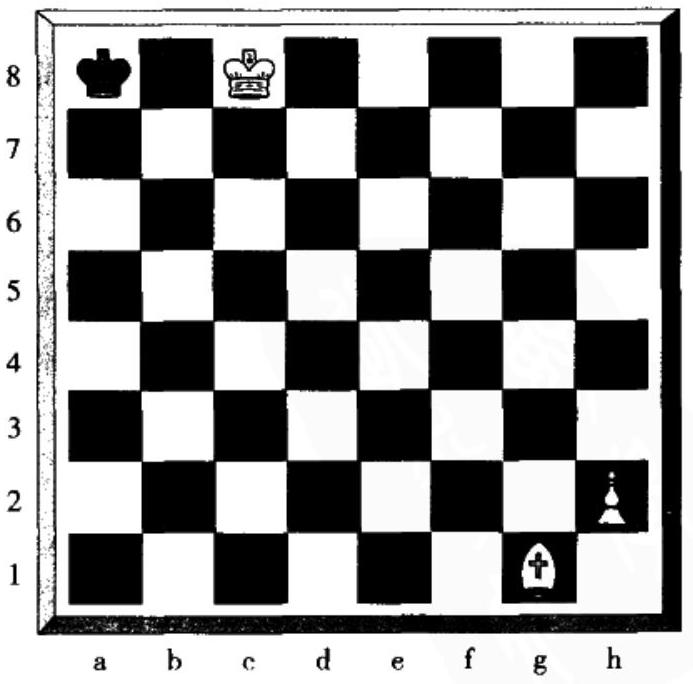
\includegraphics[width=\textwidth]{images/2025_05_15_6a28331d5e7c993ad07ag-085.jpg}

图 1-1

\begin{theorembox}[title=回溯推理过程]
\logicemph{第一步:确定黑王的前一步}
\begin{itemize}
  \item \logicterm{约束条件}:两王不能相邻
  \item \logicterm{排除法}:黑王不可能从b7或b8移动到a8
  \item \logicterm{结论}:黑王必须从a7移动到a8,且在a7时被将军
\end{itemize}

\logicemph{第二步:确定白棋的前一步}
\begin{itemize}
  \item \logicterm{问题}:什么白棋走法导致a7的黑王被将军?
  \item \logicterm{排除}:不可能是g1的白象直接将军
  \item \logicterm{推理}:必须是某个白棋子移动后,暴露了象的攻击线
  \item \logicterm{结论}:b6的马移动到a8,被黑王吃掉,同时暴露象的将军
\end{itemize}
\end{theorembox}

\logicemph{最终答案}:
\begin{itemize}
  \item 白棋最后一步:马从b6到a8
  \item 黑棋最后一步:王从a7到a8(吃掉白马)
\end{itemize}

\subsection{逻辑谜题与现实问题的对比}

虽然逻辑谜题为我们提供了优秀的推理训练,但我们必须认识到它们与现实问题之间的重要差异。

\begin{theorembox}[title=逻辑谜题与现实问题的对比]
\logicemph{逻辑谜题的特征}:
\begin{itemize}
  \item \logicterm{信息完整}:提供解决问题所需的全部信息
  \item \logicterm{描述精确}:问题陈述清晰无歧义
  \item \logicterm{答案明确}:存在确定的、可证明的解答
  \item \logicterm{封闭系统}:不需要外部信息或新发现
\end{itemize}

\logicemph{现实问题的特征}:
\begin{itemize}
  \item \logicwarn{信息不完整}:可能缺少关键信息
  \item \logicwarn{描述模糊}:问题陈述可能不精确或有歧义
  \item \logicwarn{答案开放}:可能没有唯一解或需要新发现
  \item \logicwarn{开放系统}:可能需要新的科学发现或技术突破
\end{itemize}
\end{theorembox}

\begin{theorembox}[title=现实问题的复杂性]
\logicemph{问题发现的方式}:
\begin{itemize}
  \item 往往源于矛盾现象或异常事件
  \item 基于对某种"不顺畅"的直觉感受
  \item 不是预先设计好的精确问题
\end{itemize}

\logicemph{解决的挑战}:
\begin{itemize}
  \item 可能需要重新定义问题本身
  \item 可能需要等待新的科学发现
  \item 可能需要创新的方法或工具
\end{itemize}
\end{theorembox}

\logicwarn{重要认识}:尽管存在这些差异,现实问题和逻辑谜题都需要\logicemph{系统的推理}来解决。逻辑谜题为我们提供了推理技能的训练场,而这些技能在面对现实问题时同样不可或缺。

\chaptersummary{
本章系统地介绍了逻辑学的基本概念和分析方法,为后续深入学习奠定了坚实基础。

\logicemph{核心概念}:
\begin{itemize}
  \item \logicterm{逻辑学}:研究区分正确推理与不正确推理的方法和原理
  \item \logicterm{命题}:可以肯定或否定、具有真假值的陈述
  \item \logicterm{论证}:由前提支持结论的命题集合
  \item \logicterm{演绎论证}:声称前提必然支持结论的论证
  \item \logicterm{归纳论证}:声称前提或然性支持结论的论证
\end{itemize}

\logicemph{分析方法}:
\begin{itemize}
  \item \logicterm{解析法}:按逻辑顺序列出论证中的所有命题
  \item \logicterm{图示法}:用数字和连接线展现命题间的逻辑关系
  \item \logicterm{矩阵法}:系统化处理复杂推理问题的工具
\end{itemize}

\logicemph{重要区分}:
\begin{itemize}
  \item \logicterm{论证vs说明}:证明vs解释的不同目的
  \item \logicterm{有效性vs真实性}:逻辑关系vs事实符合
  \item \logicterm{演绎vs归纳}:必然性vs或然性的支持程度
\end{itemize}

\logicemph{实践应用}:通过各种推理问题和逻辑谜题,展示了逻辑学在问题解决中的实际价值,既提供了思维训练,也带来了智力乐趣。这些技能对于日常决策、学术研究和专业工作都具有重要意义。
}

% 参考文献将在主文档末尾统一显示
